\documentclass{beamer}
\usetheme{Madrid}

\usepackage[utf8]{inputenc}
\usepackage{amsmath}
\usepackage{amsfonts}
\usepackage{amssymb}
\usepackage{graphicx}
\usepackage{xcolor}
\usepackage{tikz}

\title{CAMS Exam Preparation}
\subtitle{Complete Review of All 4 Domains (100 Slides)}
\author{Based on CAMS Candidate Handbook}
\date{}

\setbeamercovered{transparent}
\setbeamertemplate{navigation symbols}{}

\begin{document}
	
	% ============================================================
	% TITLE SLIDE
	% ============================================================
	\begin{frame}
		\titlepage
		\centering
		\textit{Domain A: 30\% | Domain B: 20\% | Domain C: 30\% | Domain D: 20\%}
	\end{frame}
	
	% ============================================================
	% DOMAIN A: UNDERSTANDING THE RISKS AND METHODS OF FINANCIAL CRIME (30%)
	% ============================================================
	
	\section{Domain A: Risks \& Methods of Financial Crime}
	
	% Subsection A.1: Definitions
	\subsection{A.1: Definitions of AML, CFT, Sanctions, Fraud, ABC, Tax Evasion}
	
	\begin{frame}{A.1.1: Money Laundering vs. Terrorist Financing}
		\begin{block}{Key Distinction (Heavily Tested)}
			\begin{itemize}
				\item \textbf{Money Laundering}: Conceals \textbf{illicit origin} of proceeds; makes funds appear legitimate. Always involves dirty money from predicate crimes.
				\item \textbf{Terrorist Financing}: Funds may be \textbf{legitimate} (donations, salary, business income); concealment objective is \textbf{intended use} for violence, not origin. Can involve very small amounts.
			\end{itemize}
		\end{block}
		\textcolor{red}{\textbf{ CRITICAL:}} Standard AML controls focused on suspicious \textbf{origins} may fail to detect TF involving \textbf{clean-source funds}. TF can involve small amounts from many donors (crowdfunding). Also, TF often moves money \textit{to} a terrorist, whereas ML moves money \textit{away from} the crime source.
	\end{frame}
	
	\begin{frame}{A.1.2: Predicate Offenses for Money Laundering}
		\begin{block}{FATF Recommendation 3 - Predicate Offenses}
			\begin{itemize}
				\item FATF recommends the \textbf{"all-crimes approach"} - applies to proceeds from \textbf{all serious criminal acts}. This is the global gold standard.
				\item \textbf{Self-laundering IS criminalized} - predicate offender can also be charged with money laundering (e.g., drug dealer washing his own cash).
				\item 6AMLD harmonizes \textbf{22 predicate offenses} across EU, including tax crimes, cybercrime, and environmental crime.
			\end{itemize}
		\end{block}
		\textcolor{blue}{Example:} Drug trafficker who processes own proceeds through a car wash business → can be charged with BOTH drug trafficking AND money laundering. No need for a separate third-party launderer.
	\end{frame}
	
	\begin{frame}{A.1.3: 6AMLD - Corporate Criminal Liability}
		\begin{block}{EU Sixth Anti-Money Laundering Directive (6AMLD)}
			\begin{itemize}
				\item \textbf{Harmonizes 22 predicate offenses} across all EU member states (binding, not optional).
				\item \textbf{Introduces criminal liability for legal persons (corporations)} - not just fines, but criminal charges.
				\item Corporation can be prosecuted and subject to: fines, debarment from public contracts, loss of subsidies, judicial supervision, dissolution.
				\item Does NOT require conviction of individual directors first (entity can be liable independently).
				\item Extends liability to negligent supervisors who fail to prevent ML.
			\end{itemize}
		\end{block}
		\textcolor{red}{\textbf{TIP:}} 6AMLD is \textbf{heavily tested} - know the difference from 5AMLD (5AMLD added VASPs and lowered prepaid card thresholds from EUR 250 to EUR 150).
	\end{frame}
	
	% Subsection A.2: Financial Systems and Consequences
	\subsection{A.2: Economic and Social Consequences of ML}
	
	\begin{frame}{A.2.1: Consequences of Money Laundering}
		\begin{columns}
			\column{0.5\textwidth}
			\textbf{Economic Consequences}
			\begin{itemize}
				\item Distorts markets and asset prices (artificial demand)
				\item Undermines legitimate private sector (unfair competition)
				\item Loss of tax revenue for governments
				\item Reputational damage to financial centers (capital flight)
				\item Misallocation of resources (real estate bubbles)
			\end{itemize}
			\column{0.5\textwidth}
			\textbf{Social Consequences}
			\begin{itemize}
				\item Funds criminal enterprises (drugs, trafficking, arms)
				\item Corruption of public officials and erosion of trust
				\item Erodes rule of law and democratic institutions
				\item Fuels violence, instability, and terrorism
				\item Increases poverty and inequality
			\end{itemize}
		\end{columns}
	\end{frame}
	
	\begin{frame}{A.2.2: Consequences of Indiscriminate De-Risking}
		\begin{block}{De-Risking Definition}
			Termination of entire categories of customer relationships without individual risk assessment (e.g., "no more MSBs" or "no more Caribbean correspondents").
		\end{block}
		\textbf{Negative Consequences (Heavily Tested):}
		\begin{itemize}
			\item Legitimate businesses lose access to global financial system (e.g., remittance corridors for migrant workers).
			\item Drives transactions into \textbf{unregulated, informal channels} (e.g., hawala, crypto mixers) which are harder to monitor.
			\item Harms financial inclusion and developing economies (remittances are lifelines).
			\item Contradicts the mandatory \textbf{risk-based approach} required by FATF.
		\end{itemize}
		\textcolor{red}{\textbf{FATF \& Wolfsberg guidance:}} Individual, documented risk assessments required - NOT blanket exclusions. Exiting a relationship must be based on documented unacceptable residual risk.
	\end{frame}
	
	% Subsection A.3: Predicate Crimes
	\subsection{A.3: Predicate Crimes Underlying Financial Crime}
	
	\begin{frame}{A.3.1: Self-Laundering and Double Jeopardy}
		\begin{block}{Self-Laundering (18 U.S.C. §1956)}
			\begin{itemize}
				\item U.S. law \textbf{DOES} criminalize self-laundering (unlike some civil law jurisdictions historically).
				\item Predicate offender CAN be charged with money laundering for processing own proceeds (e.g., spending drug money on real estate).
				\item \textbf{Double jeopardy argument fails} - each offense requires proof of different elements (predicate crime + financial transaction with intent to conceal).
			\end{itemize}
		\end{block}
		\begin{example}
			Wire fraud (predicate: deceptive scheme) + money laundering of proceeds (financial transaction to conceal source) = TWO separate crimes with distinct elements. Consecutive sentences possible.
		\end{example}
	\end{frame}
	
	% Subsection A.4: ML/TF Manifestations Across Sectors
	\subsection{A.4: ML/TF Manifestations Across Sectors}
	
	\begin{frame}{A.4.1: Trade-Based Money Laundering (TBML)}
		\begin{block}{TBML Techniques (Heavily Tested)}
			\begin{itemize}
				\item \textbf{Over-invoicing}: Inflated prices → transfer excess value from importer to exporter (exporter overstates value, receives excess payment).
				\item \textbf{Under-invoicing}: Deflated prices → importer sells at market price, keeps surplus as "clean" funds (understates value, pays less, resells at true value).
				\item \textbf{Phantom shipping}: No actual goods; fabricated documentation (bill of lading, invoices) to move money.
				\item \textbf{Multiple invoicing}: Same goods invoiced multiple times, often through different banks.
				\item \textbf{Short-shipping/over-shipping}: Discrepancy between invoice quantity and actual shipped goods.
			\end{itemize}
		\end{block}
		\vspace{0.2cm}
		\textcolor{red}{\textbf{ Red flags:}} Prices significantly above/below market (e.g., 400\% premium), shell company exporter, multiple L/C amendments, circuitous shipping routes, goods inconsistent with exporter's normal business.
	\end{frame}
	
	\begin{frame}{A.4.2: Free Trade Zone (FTZ) Vulnerabilities}
		\begin{block}{Why FTZs are High Risk}
			\begin{itemize}
				\item \textbf{Relaxed regulatory oversight} (customs and AML controls minimal).
				\item Minimal customs documentation inspections (goods in transit often not examined).
				\item High volume of re-exported goods (obscures origin and destination).
				\item Opportunity for mislabeling cargo (e.g., electronics labeled as scrap).
				\item Phantom shipments (no goods, just paperwork).
				\item Presence of shell companies and nominee directors.
			\end{itemize}
		\end{block}
		\textbf{Red flags:} Uniform invoice values regardless of cargo (all \$50,000), empty containers, altered bills of lading, nominee directors, goods remaining in FTZ far longer than normal.
	\end{frame}
	
	\begin{frame}{A.4.3: Black Market Peso Exchange (BMPE)}
		\begin{block}{BMPE Mechanism (Heavily Tested)}
			\begin{enumerate}
				\item Narco-dollars deposited in U.S. accounts (often structured below 10k).
				\item Colombian peso broker buys those dollars at a discount (e.g., 20-30\% below official rate).
				\item Broker uses dollars to pay U.S. invoices for Colombian merchants (legitimate goods like electronics, clothing).
				\item Colombian merchant repays broker in pesos (at favorable rate, often above market).
				\item \textbf{No cross-border currency movement} after initial deposit; drug dollars become pesos without leaving Colombia officially.
			\end{enumerate}
		\end{block}
		\textbf{Key insight:} Uses drug dollars to pay legitimate commercial invoices; converts narco-dollars into domestic pesos without wire transfers. The broker profits on the exchange rate spread.
	\end{frame}
	
	\begin{frame}{A.4.4: Black Market Peso Exchange - Diagram}
		\begin{center}
			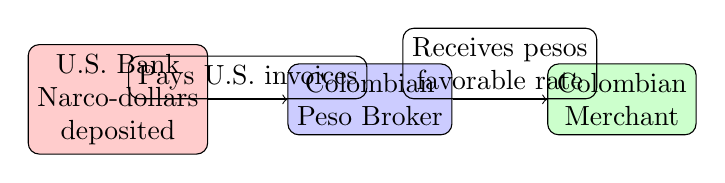
\begin{tikzpicture}[scale=0.8, every node/.style={draw, rounded corners, align=center}]
				\node[fill=red!20] (US) at (0,0) {U.S. Bank\\Narco-dollars\\deposited};
				\node[fill=blue!20] (Broker) at (4,0) {Colombian\\Peso Broker};
				\node[fill=green!20] (Merchant) at (8,0) {Colombian\\Merchant};
				\draw[->] (US) -- (Broker) node[midway, above] {Pays U.S. invoices};
				\draw[->] (Broker) -- (Merchant) node[midway, above] {Receives pesos\\favorable rate};
			\end{tikzpicture}
		\end{center}
		\textbf{No wire transfers!} The scheme uses \textbf{existing U.S. dollars} to pay legitimate invoices, avoiding cross-border movement. Detection requires analyzing unusual trade invoices and structured cash deposits.
	\end{frame}
	
	% Subsection A.5: Banking Sector Product Risks
	\subsection{A.5: Banking Sector Product Risks}
	
	\begin{frame}{A.5.1: Correspondent Banking Risks}
		\begin{block}{Nested Correspondent Accounts - Critical Risk}
			When a respondent bank allows third parties (e.g., its own customers, other smaller banks, MSBs) to route transactions through the correspondent account \textbf{without disclosure}:
			\begin{itemize}
				\item Correspondent bank loses visibility into true originators/beneficiaries (only sees respondent as sender/receiver).
				\item Increased risk of processing for sanctioned entities or illicit actors.
				\item Violates core KYC and correspondent banking due diligence (CDD on underlying users is missing).
			\end{itemize}
		\end{block}
		\textbf{Required actions:} Immediate RFI to respondent, SAR filing if suspicious, reassess relationship, potentially terminate if no adequate response.
	\end{frame}
	
	\begin{frame}{A.5.2: Payable-Through Accounts (PTAs)}
		\begin{block}{PTA Obligations (U.S. Regulations)}
			\begin{itemize}
				\item Correspondent bank MUST apply CDD directly to respondent's underlying PTA accountholders (cannot delegate).
				\item Must maintain records identifying each PTA accountholder (name, address, tax ID).
				\item \textbf{Cannot rely solely on respondent's CDD} - must perform own due diligence on those using the PTA.
			\end{itemize}
		\end{block}
		\textbf{Red flag:} Multiple sub-\$10,000 wires from different PTA accountholders to same shell company → possible structuring/money mule activity. Also, rapid in-and-out flows with no business purpose.
	\end{frame}
	
	% Subsection A.6: High-Risk Sector Banking
	\subsection{A.6: High-Risk Sector Banking}
	
	\begin{frame}{A.6.1: MSB Agent Network Risk}
		\begin{block}{MSB Principal Responsibility}
			\begin{itemize}
				\item MSB principal is \textbf{responsible for agent network compliance} under BSA (e.g., MoneyGram for its corner store agents).
				\item Unexplained volume spikes require investigation (e.g., agent does \$5M/month when historical \$100k).
				\item SAR filing on agent location may be required for suspicious activity (not just on customers).
				\item Agent termination if compliance cannot be ensured (e.g., refuses monitoring, falsifies records).
			\end{itemize}
		\end{block}
		\textbf{Red flag:} Agent processes 5,000\% above historical average → all transfers under \$900 (just below CTR), same destination countries, same customer phone number repeated across senders.
	\end{frame}
	
	% Subsection A.7: PEP and High-Risk Customer Banking
	\subsection{A.7: PEP and High-Risk Customer Banking}
	
	\begin{frame}{A.7.1: PEP Definition and Family Members}
		\begin{block}{PEP Classification (FATF)}
			\textbf{Who qualifies as PEP:}
			\begin{itemize}
				\item Foreign heads of state/government (presidents, prime ministers)
				\item Senior politicians, cabinet ministers, senior parliamentarians
				\item Senior judicial officials (supreme court justices, constitutional court)
				\item Senior military officials (generals, admirals)
				\item Senior executives of state-owned enterprises (CEOs of national oil companies)
				\item \textbf{Family members and close associates} of the above (spouse, children, parents, siblings, known business partners)
			\end{itemize}
		\end{block}
		\textcolor{red}{\textbf{Critical:}} Adult child of a foreign minister \textbf{IS a PEP family member} requiring EDD, even with no government position. Close associate who jointly owns a company with a PEP is also a PEP.
	\end{frame}
	
	\begin{frame}{A.7.2: PEP Lifecycle Management}
		\begin{block}{When a Customer Becomes a PEP (Mid-Relationship)}
			\begin{itemize}
				\item \textbf{Immediate reclassification to HIGH risk} (no delay, no grace period).
				\item Mandatory Enhanced Due Diligence (EDD) applied within days, not months.
				\item Re-establish and verify source of wealth AND source of funds (new documentation required).
				\item Senior management approval to continue relationship (documented sign-off).
				\item Back-dated gap period is a control failure (e.g., "we knew but didn't act for 6 months" is violation).
			\end{itemize}
		\end{block}
		\textcolor{blue}{Example:} Customer elected to foreign cabinet → bank must re-rate immediately, NOT wait for scheduled annual review. Apply EDD to all existing accounts and transactions.
	\end{frame}
	
	\begin{frame}{A.7.3: Former PEP - Grace Period}
		\begin{block}{PEP Status After Retirement}
			\begin{itemize}
				\item FATF: maintain PEP status for \textbf{"reasonable period"} (minimum 12 months recommended).
				\item \textbf{Risk-based decision} - consider country corruption risk, continued informal influence, business connections to current PEPs.
				\item 5 years clean activity (no red flags, transparent wealth) MAY justify lowering to medium or standard risk.
				\item \textbf{Must be documented} with rationale for any change.
			\end{itemize}
		\end{block}
		\textcolor{red}{\textbf{}} No automatic rule; each decision must be documented with risk rationale. A former president of a high-corruption country may remain PEP for life.
	\end{frame}
	
	\begin{frame}{A.7.4: EDD - Source of Wealth vs. Source of Funds}
		\begin{block}{Critical Distinction (Heavily Tested)}
			\begin{itemize}
				\item \textbf{Source of Funds (SoF)}: Specific transaction being deposited (e.g., property sale contract showing proceeds from buyer, inheritance letter, business dividend voucher).
				\item \textbf{Source of Wealth (SoW)}: How PEP accumulated \textbf{overall net worth} over time (career earnings, inheritance, business ownership, investments, gifts).
			\end{itemize}
		\end{block}
		\textcolor{red}{\textbf{ EDD for PEPs requires BOTH.}} A lifelong civil servant with a \$4.5M Paris apartment → SoF document (sale contract) insufficient without SoW showing how she could afford to buy it. Must trace back to legitimate income, gift, inheritance, or loan.
	\end{frame}
	
	% Subsection A.8: Other Financial Sectors
	\subsection{A.8: Other Financial Sector Risks}
	
	\begin{frame}{A.8.1: Life Insurance ML Vulnerabilities}
		\begin{block}{CDD Triggers for Life Insurance}
			\begin{itemize}
				\item Premium > USD/EUR 10,000 per year OR single premium > USD/EUR 10,000 triggers CDD.
				\item Must apply CDD to \textbf{policyholder AND beneficiary} (once beneficiary is designated, possibly later).
			\end{itemize}
		\end{block}
		\textbf{Exploitation methods:}
		\begin{itemize}
			\item Policy loan feature = layering (convert dirty premium to "legitimate" loan check, then surrender).
			\item Cash surrender value extraction after brief holding period (e.g., 6 months, pay penalty but get clean check).
			\item Premiums from secrecy haven jurisdiction + offshore shell company beneficiary = red flags for TF or ML.
		\end{itemize}
	\end{frame}
	
	% Subsection A.9: MSBs, PSPs, E-commerce
	\subsection{A.9: MSBs, PSPs, E-commerce Risks}
	
	\begin{frame}{A.9.1: MSB Registration Triggers (U.S.)}
		\begin{block}{Who Must Register as MSB with FinCEN}
			\begin{itemize}
				\item Check casher cashing > \$1,000 per person per day (any day).
				\item Money transmitter (any volume, including crypto-to-fiat and fiat-to-crypto).
				\item Currency dealer or exchanger (forex, crypto if exchanging).
				\item Issuer or seller of prepaid access (stored value cards).
				\item Traveler's check issuer.
			\end{itemize}
		\end{block}
		\textcolor{red}{\textbf{}} Grocery store cashing checks > \$1,000/day without registration = BSA violation. "No ID required" policy + MSB services = ML vulnerability (anonymous transactions).
	\end{frame}
	
	% Subsection A.10: Insurance Products
	\subsection{A.10: Insurance Product Risks}
	
	\begin{frame}{A.10.1: Insurance Red Flags}
		\begin{block}{Life Insurance ML Indicators}
			\begin{itemize}
				\item Single premium payment from offshore shell company (no legitimate business reason).
				\item Early surrender (e.g., 60 days) with proceeds sent to a different bank account than premium source.
				\item Policyholder is foreign PEP; beneficiary is offshore shell company.
				\item Premium from secrecy haven jurisdiction (e.g., Caymans, Panama, with no economic substance).
				\item Large premium relative to legitimate income (e.g., janitor buys \$2M policy).
			\end{itemize}
		\end{block}
		\textbf{Layering technique:} Purchase policy (placement) → take policy loan (layering: dirty money becomes "loan" on books) → wire to offshore account (further layering) → surrender policy (integration: get check minus penalty).
	\end{frame}
	
	% Subsection A.11: VASPs and Cryptoassets
	\subsection{A.11: VASPs and Cryptoassets}
	
	\begin{frame}{A.11.1: FATF Travel Rule for VASPs}
		\begin{block}{Virtual Asset Travel Rule (Recommendation 16)}
			\textbf{Required information for transfers above threshold (USD/EUR 1,000):}
			\begin{itemize}
				\item Originator: name, account number/wallet ID (or unique transaction identifier).
				\item Originator: address, national ID, customer ID, or DOB (at least ONE of these three).
				\item Beneficiary: name and account number/wallet ID.
			\end{itemize}
		\end{block}
		\textcolor{red}{\textbf{ Receiving VASP obligations:}} Must obtain and hold info; if not provided → follow up, delay transaction (e.g., 24 hours), apply EDD, consider SAR. Non-compliance is a regulatory violation.
	\end{frame}
	
	\begin{frame}{A.11.2: DeFi and AML Responsibility}
		\begin{block}{FATF DeFi Guidance - Critical Point}
			If a person/entity maintains \textbf{control or sufficient influence} over a DeFi protocol:
			\begin{itemize}
				\item Through governance token majority (>50\% of voting power).
				\item Ability to upgrade contract code (admin keys, multi-sig control).
				\item Ongoing management/control (fees, parameters, user access).
			\end{itemize}
			\vspace{0.2cm}
			\textcolor{red}{\textbf{They may be considered a VASP}} subject to registration, KYC, transaction monitoring, and SAR filing obligations. "Decentralized in name only" is not a defense.
		\end{block}
		\textbf{Example:} 5 founders retain 68\% governance tokens and control code upgrades → likely subject to AML obligations as a VASP.
	\end{frame}
	
	\begin{frame}{A.11.3: Privacy Coins and Mixers}
		\begin{block}{Anonymity-Enhanced Cryptocurrencies (AECs)}
			\textbf{Monero (XMR) risk features:}
			\begin{itemize}
				\item Ring signatures (obscures which input is real) and stealth addresses (one-time addresses per transaction).
				\item Can be used with mixers/tumblers (e.g., Wasabi, Tornado Cash) to further obfuscate trail.
			\end{itemize}
		\end{block}
		\textbf{Red flags requiring EDD/SAR:}
		\begin{itemize}
			\item Customer deposits privacy coin → immediately exchanges for BTC/ETH → sends to non-custodial wallet → refuses to explain source.
			\item Funds sent through non-regulated mixer before deposit (chain hop pattern).
			\item Customer claims "privacy protection" without legitimate business explanation (e.g., no need for a grocery store to use Monero).
		\end{itemize}
	\end{frame}
	
	\begin{frame}{A.11.4: NFT Wash Trading}
		\begin{block}{NFT Wash Trading Typology}
			\begin{enumerate}
				\item Self-controlled wallets (e.g., 5-20 wallets owned by same person) buy/sell same NFTs among themselves.
				\item Prices artificially escalate through circular transactions (e.g., 2k -> $50k -> $200k).
				\item Creates fraudulent market record (looks like high demand).
				\item Sells NFT to unwitting third party at inflated price.
				\item Converts to fiat, reports as "capital gain" for tax purposes, laundering the original illicit funds.
			\end{enumerate}
		\end{block}
		\textbf{Exchange obligation:} File SAR based on wash trading pattern regardless of whether underlying proceeds from predicate crime. Pattern detection is key.
	\end{frame}
	
	% Subsection A.12: Gaming and Gambling
	\subsection{A.12: Gaming and Gambling Risks}
	
	\begin{frame}{A.12.1: Casino Chip Washing}
		\begin{block}{Chip Washing Scheme}
			\textbf{Pattern:}
			\begin{itemize}
				\item Large cash purchase of chips (>\$10,000, triggers CTR).
				\item Minimal gaming (e.g., 45 minutes, \$1,500 played, mostly low-risk bets).
				\item Cash out rest for casino check (clean paper trail).
				\item Accepts small "gaming loss" (e.g., \$500) as cost of laundering (like a fee).
			\end{itemize}
		\end{block}
		\textbf{Obligations:} File CTR for cash-in + SAR (chip washing pattern if gaming disproportionate to buy-in) → combined placement (cash to chips) and integration (check from casino). Also check if chip purchases made by third party.
	\end{frame}
	
	\begin{frame}{A.12.2: Online Gaming ML}
		\begin{block}{In-Game Currency Laundering}
			\textbf{Stages:}
			\begin{enumerate}
				\item \textbf{Placement}: Purchase in-game currency (e.g., V-Bucks, Gold) with criminal cash via prepaid cards or crypto.
				\item \textbf{Layering}: Distribute across multiple gamer accounts (trade among themselves).
				\item \textbf{Integration}: Sell currency peer-to-peer (e.g., eBay, Discord) for PayPal or bank transfer, deposit to clean accounts as "gaming income" or "digital asset sale."
			\end{enumerate}
		\end{block}
		\textbf{Difficulty:} Small individual transactions (\$200-\$800) fall below reporting thresholds (e.g., \$3k for PayPal in some jurisdictions); requires pattern recognition across many small sells.
	\end{frame}
	
	% Subsection A.13: Real Estate
	\subsection{A.13: Real Estate Risks}
	
	\begin{frame}{A.13.1: FinCEN Geographic Targeting Orders (GTOs)}
		\begin{block}{GTO Requirements}
			\begin{itemize}
				\item Title insurance companies must identify \textbf{natural persons behind legal entities} (LLCs, trusts, corporations) buying residential real estate.
				\item All-cash purchases above threshold (\$300,000 in designated metro areas; varies by area).
				\item Target specific metropolitan areas (Miami, LA, NYC, Chicago, Seattle, Las Vegas, etc.).
				\item \textbf{Temporary} orders, renewed periodically (every 6-12 months).
			\end{itemize}
		\end{block}
		\textbf{Red flags:} Recently formed LLC (e.g., 2 weeks before closing), IOLTA wire (attorney trust account), registered agent refuses to disclose UBO → decline closing until UBO identified and verified.
	\end{frame}
	
	\begin{frame}{A.13.2: Real Estate Integration}
		\begin{block}{Real Estate as Integration Vehicle}
			\textbf{Example scheme:}
			\begin{enumerate}
				\item Structured cash deposits (placement, under \$10k each at multiple banks).
				\item Purchase property via anonymous LLC (layering, hides true buyer).
				\item Rent property, report rental income on taxes (integration: funds now appear legitimate from a legal business).
			\end{enumerate}
		\end{block}
		\textbf{Red flags for acquiring bank when property sold (e.g., after 2 years):}
		\begin{itemize}
			\item Rapid appreciation (e.g., \$9.5M to \$12M in 18 months in normal market).
			\item Original purchase by anonymous LLC with no obvious source of funds.
			\item Wire proceeds to secrecy haven account (Caymans, Switzerland) immediately after sale.
			\item No verified source of acquisition funds at time of sale (bank didn't ask).
		\end{itemize}
	\end{frame}
	
	% Subsection A.14: Gatekeepers
	\subsection{A.14: Gatekeeper Risks}
	
	\begin{frame}{A.14.1: IOLTA Account Vulnerabilities}
		\begin{block}{Why IOLTA Accounts Are Dangerous}
			\begin{itemize}
				\item Banks rely on attorney's professional status (presume legitimate).
				\item \textbf{Do NOT look through} pooled account to identify individual client sub-transactions (lack of granular monitoring).
				\item Illicit funds enter credentialed by attorney status (seems legitimate).
				\item Commingled with legitimate client funds (makes tracing hard).
				\item Rapid disbursement possible (attorney can move funds quickly to third parties).
			\end{itemize}
		\end{block}
		\textbf{Red flags:} Wire from shell company to IOLTA (no prior relationship), retainer disproportionate to transaction (e.g., $500k retainer for $50k real estate deal), no face-to-face contact (client from high-risk jurisdiction), rapid disbursement to offshore or unrelated third parties.
	\end{frame}
	
	% Subsection A.15: Trusts and Company Service Providers
	\subsection{A.15: Trusts and Company Service Providers}
	
	\begin{frame}{A.15.1: Trust Beneficial Ownership}
		\begin{block}{Trust CDD Requirements (FATF)}
			Must identify and verify:
			\begin{itemize}
				\item Settlor (person who creates the trust and contributes assets).
				\item Trustee (and its UBOs if corporate trustee like a trust company).
				\item \textbf{Protector} (if has veto, replacement rights, or power to direct distributions).
				\item Beneficiaries (to extent determinable - named individuals or defined class).
			\end{itemize}
		\end{block}
		\textcolor{red}{\textbf{}} Protector with veto over distributions qualifies as PEP if former head of state → entire trust becomes high risk requiring EDD. Bank must look through to each role.
	\end{frame}
	
	\begin{frame}{A.15.2: Bearer Shares Risk}
		\begin{block}{Bearer Shares - Highest Vulnerability}
			\begin{itemize}
				\item Ownership transferred by physical delivery of certificate (whoever holds the paper owns the shares).
				\item \textbf{NO public registry record} of who owns the company.
				\item FATF Recommendation 24: prohibit or require immobilization with regulated custodian (e.g., bank, licensed agent).
			\end{itemize}
		\end{block}
		\textbf{Bank obligations:}
		\begin{itemize}
			\item Verify custodian can identify bearer share holder at all times (must have recorded transfers).
			\item Still need to identify UBO for CDD regardless of immobilization (ask custodian for name).
			\item Decline account if custodian refuses to disclose UBO (cannot accept anonymous ownership).
		\end{itemize}
	\end{frame}
	
	% Subsection A.16: Accountants
	\subsection{A.16: Accountant Risks}
	
	\begin{frame}{A.16.1: Financial Statement Manipulation}
		\begin{block}{Red Flags Involving Accountants}
			\begin{itemize}
				\item Financial statements inconsistent with bank statements (e.g., reported revenue \$10M, deposits \$2M).
				\item Unusually high "consulting fees" or "services" with no deliverables or contracts.
				\item Client cannot explain discrepancy between reported income and cash flow (e.g., tax return shows \$500k income, lifestyle shows \$5M spending).
				\item Auditor unwilling to verify underlying records (e.g., "we trust management").
			\end{itemize}
		\end{block}
		\textbf{Bank action:} Verify underlying records (e.g., sales invoices, contracts) directly with customer; do NOT rely solely on accountant-prepared financial statements. SAR if discrepancy unexplained.
	\end{frame}
	
	% Subsection A.17: Other High-Risk Sectors
	\subsection{A.17: Other High-Risk Sectors}
	
	\begin{frame}{A.17.1: Human Trafficking Financial Indicators}
		\begin{block}{Trafficking Red Flags (Heavily Tested)}
			\begin{itemize}
				\item Multiple individuals sending small payments to single controller account (e.g., 50 people send \$200 each monthly).
				\item Controller pays utilities for multiple residential addresses (electric, water, internet for different houses).
				\item Weekly cash withdrawal of 85-95\% of balance (victims get minimal spending money).
				\item No employment contracts or payroll records for apparent workers.
				\item Victims share same surname as controller (family-based trafficking).
				\item Large number of transactions at odd hours (e.g., 2 AM in massage parlors, nail salons).
			\end{itemize}
		\end{block}
		\textbf{vs. Human Smuggling:} Trafficking = ongoing exploitation (forced labor, sexual); Smuggling = one-time fee for illegal border crossing (ends at destination).
	\end{frame}
	
	\begin{frame}{A.17.2: NPO Terrorist Financing Vulnerabilities}
		\begin{block}{FATF Recommendation 8 - NPO Risks}
			\textbf{Vulnerabilities:}
			\begin{itemize}
				\item Operate in conflict zones with weak financial monitoring (Syria, Yemen, Somalia).
				\item Enjoy public trust, receive large cash donations (often anonymous).
				\item Limited scrutiny of fund utilization (donors don't audit).
				\item Cash withdrawals inconsistent with stated mission (e.g., food charity making large cash withdrawals near conflict zone).
			\end{itemize}
		\end{block}
		\textbf{Red flags:} Large donation from Grey List jurisdiction (e.g., 1M from high-risk country), rapid cash withdrawal far from HQ (80\% in 48 hours across country), transfers to conflict zone sub-NPOs where terrorists control aid distribution.
	\end{frame}
	
	% ============================================================
	% DOMAIN B: GLOBAL AFC FRAMEWORKS, GOVERNANCE, REGULATIONS (20%)
	% ============================================================
	
	\section{Domain B: Global AFC Frameworks \& Regulations}
	
	% Subsection B.1: FATF Role and Recommendations
	\subsection{B.1: FATF Role, Function, and Recommendations}
	
	\begin{frame}{B.1.1: FATF Mutual Evaluation - Two Pillars}
		\begin{block}{Technical Compliance vs. Effectiveness}
			\begin{itemize}
				\item \textbf{Technical Compliance}: Do laws exist on paper? (40 Recommendations rated compliant, largely compliant, partially compliant, non-compliant).
				\item \textbf{Effectiveness}: Do laws achieve intended outcomes? (11 Immediate Outcomes rated high, substantial, moderate, low).
			\end{itemize}
		\end{block}
		\textcolor{red}{\textbf{ Critical:}} A country can have \textbf{perfect technical compliance} (all laws in place) but \textbf{Low effectiveness} if:
		\begin{itemize}
			\item FIU never disseminates intelligence to law enforcement (reports sit on server).
			\item Zero ML convictions despite high predicate crime (e.g., drug trafficking).
			\item No asset forfeitures (no money recovered).
		\end{itemize}
	\end{frame}
	
	\begin{frame}{B.1.2: FATF Immediate Outcomes (IO.1-IO.11)}
		\begin{block}{Key Immediate Outcomes (Heavily Tested)}
			\begin{itemize}
				\item \textbf{IO.1}: ML/TF risks understood and coordinated domestically (national risk assessment exists and is used).
				\item \textbf{IO.6}: Financial intelligence used by competent authorities (FIU reports lead to investigations).
				\item \textbf{IO.7}: ML investigated and prosecuted (actual convictions, not just charges).
				\item \textbf{IO.8}: Proceeds of crime confiscated (assets recovered, not just restrained).
				\item \textbf{IO.10}: TF investigated and prosecuted (standalone TF cases, not just ML).
			\end{itemize}
		\end{block}
		\textbf{Evidence for IO.1:} Regular NRA (every 3-5 years) that drives resource allocation (e.g., budget for high-risk sectors), NOT just existence of laws.
	\end{frame}
	
	\begin{frame}{B.1.3: FATF Grey List vs. Black List}
		\begin{block}{Grey List - Increased Monitoring (e.g., Turkey, Jamaica, Albania)}
			\begin{itemize}
				\item Committed to action plan with specific deadlines (e.g., improve beneficial ownership registry, increase ML prosecutions).
				\item Financial institutions should apply EDD to transactions involving grey list countries.
				\item NOT automatically required to terminate relationships (risk-based: assess individually).
				\item Individual risk assessments required (e.g., customer doing legitimate business vs. shell company).
			\end{itemize}
		\end{block}
		\begin{block}{Black List - Call for Action (e.g., Iran, North Korea)}
			\begin{itemize}
				\item Strategic deficiencies (e.g., no AML regime, no TF criminalization).
				\item Apply \textbf{countermeasures} (e.g., enhanced scrutiny, restrictions, or termination).
				\item FATF calls on members to apply enhanced due diligence or countermeasures.
			\end{itemize}
		\end{block}
	\end{frame}
	
	\begin{frame}{B.1.4: FATF Recommendation 16 - Wire Transfer Rule}
		\begin{block}{Required Information (Cross-border > USD 1,000)}
			\textbf{Originator:}
			\begin{itemize}
				\item Full name (legal name, no initials).
				\item Account number (or unique reference if no account).
				\item Address (residential or business), national ID number, customer ID number, OR date and place of birth (at least ONE of these).
			\end{itemize}
			\textbf{Beneficiary:}
			\begin{itemize}
				\item Full name.
				\item Account number (or unique identifier).
			\end{itemize}
		\end{block}
		\textcolor{red}{\textbf{Most critical violation:}} Omitting ALL three qualifying identifiers (address, ID, DOB) for originator when sending wire over \$1,000.
	\end{frame}
	
	\begin{frame}{B.1.5: FATF Recommendation 10 - CDD Triggers}
		\begin{block}{When CDD Must Be Conducted}
			\begin{enumerate}
				\item Establishing business relationship (before or during onboarding).
				\item Occasional transaction above threshold (USD/EUR 15,000 or local equivalent).
				\item Suspicion of ML/TF (regardless of amount, even \$10).
				\item Doubt about veracity of previously obtained ID (e.g., fuzzy copy, mismatch).
			\end{enumerate}
		\end{block}
		\textbf{CDD elements:} 1) Identify customer (name, DOB, address), 2) Verify ID (documentary or electronic), 3) Identify beneficial owner (natural person), 4) Understand purpose and intended nature (expected activity), 5) Ongoing monitoring (refresh, transaction screening).
	\end{frame}
	
	\begin{frame}{B.1.6: FATF Recommendation 1 - Risk-Based Approach}
		\begin{block}{RBA Principles}
			\begin{itemize}
				\item Identify, assess, understand ML/TF risks (jurisdictional, sectoral, customer, product).
				\item Apply measures \textbf{commensurate with risks} (high risk = EDD, low risk = SDD).
				\item Simplified measures where risks are lower (e.g., capped accounts, basic products, low-risk geography).
				\item Enhanced measures where risks are higher (PEPs, high-risk jurisdictions, complex structures).
				\item \textbf{NOT} zero-risk tolerance (impossible; objective is managed risk).
			\end{itemize}
		\end{block}
		\textcolor{blue}{Contrast with rules-based approach:} RBA is more effective and efficient; concentrates resources on highest risks rather than applying same controls everywhere.
	\end{frame}
	
	\begin{frame}{B.1.7: FATF Recommendation 3 - Money Laundering Offense}
		\begin{block}{Key Requirements}
			\begin{itemize}
				\item Apply to \textbf{all serious predicate offenses} (all-crimes approach preferred; at minimum, 22 designated categories including drug trafficking, fraud, corruption, tax crimes, environmental crime).
				\item Apply to \textbf{self-laundering} (predicate offender can be charged separately; no third-party launderer needed).
				\item Apply regardless of whether predicate offense occurred in another jurisdiction (extraterritorial application).
			\end{itemize}
		\end{block}
		\textbf{Minimum predicate offenses:} At least designated categories including drug trafficking, fraud, corruption, tax crimes. Countries can add more.
	\end{frame}
	
	\begin{frame}{B.1.8: FATF Recommendation 5 - Terrorist Financing Offense}
		\begin{block}{TF Offense Requirements}
			\begin{itemize}
				\item Criminalize TF regardless of whether funds actually used for terrorist act (attempt or conspiracy sufficient).
				\item \textbf{No minimum monetary threshold} (even 1 is enough).
				\item Collection of funds for terrorist purposes is sufficient (fundraising for designated terrorist group).
				\item Standalone offense (not just covered under ML; separate statute or section).
			\end{itemize}
		\end{block}
		\textcolor{red}{\textbf{ Deficiency:}} \$10,000 threshold for TF violates Recommendation 5 (implies small amounts are legal). Zero convictions despite known TF activity = low effectiveness on IO.10.
	\end{frame}
	
	\begin{frame}{B.1.9: FATF Recommendation 8 - NPOs}
		\begin{block}{NPO Obligations}
			\begin{itemize}
				\item Apply targeted risk-based supervision of NPOs vulnerable to TF (not all NPOs, only high-risk subset).
				\item Mechanisms to prevent NPO misuse by terrorist organizations (e.g., donor verification, fund tracking).
				\item Outreach, supervision, monitoring of cross-border transactions (e.g., suspicious wire to conflict zone).
			\end{itemize}
		\end{block}
		\textbf{NOT exempt:} Conflict zone NPOs are HIGH risk, not exempt from scrutiny. Cash withdrawal velocity mismatch with charitable mission (e.g., \$500k withdrawn in 48 hours for "food aid" but no food purchased) = red flag.
	\end{frame}
	
	\begin{frame}{B.1.10: FATF Recommendation 14 - MVTS (Hawala)}
		\begin{block}{Money or Value Transfer Services}
			\begin{itemize}
				\item Must be licensed or registered (no unlicensed operators).
				\item Subject to AML/CFT monitoring (CDD, recordkeeping, STR filing).
				\item Unlicensed providers subject to sanctions (criminal or administrative penalties).
				\item \textbf{No cultural heritage exemption} for hawala (traditional but still regulated).
			\end{itemize}
		\end{block}
		\textbf{Hawala risks:} Trust-based settlement (honor system), no traceable banking record (only logbooks), no CDD (often nickname based), no SAR filing (underground).
	\end{frame}
	
	\begin{frame}{B.1.11: FATF Recommendation 15 - New Technologies}
		\begin{block}{Virtual Assets and VASPs}
			\begin{itemize}
				\item Countries must assess ML/TF risks of new technologies (e.g., DeFi, privacy coins, NFTs).
				\item VASPs must be licensed or registered (crypto exchanges, custodial wallet providers).
				\item Subject to AML/CFT obligations (CDD, Travel Rule, recordkeeping, SAR filing).
				\item \textbf{No exemption} for DeFi if control exists (see earlier DeFi slide).
			\end{itemize}
		\end{block}
		\textbf{Applies to:} Crypto exchanges (CEX), custodian wallet providers, certain DeFi protocols with admin keys, OTC desks, some NFT platforms if they facilitate value transfer.
	\end{frame}
	
	\begin{frame}{B.1.12: FATF Recommendation 19 - High-Risk Jurisdictions}
		\begin{block}{Response to FATF-Designated High-Risk Jurisdictions}
			\textbf{Black List (Call for Action - Iran, North Korea):}
			\begin{itemize}
				\item Apply EDD to relationships and transactions (enhanced scrutiny).
				\item Apply countermeasures (may include restricting, limiting, or terminating correspondent relationships).
			\end{itemize}
			\textbf{Grey List (Increased Monitoring - e.g., Turkey, Jamaica):}
			\begin{itemize}
				\item Apply EDD (enhanced scrutiny).
				\item Countermeasures not automatically required (risk-based).
				\item Individual risk assessments (customer-by-customer).
			\end{itemize}
		\end{block}
	\end{frame}
	
	\begin{frame}{B.1.13: FATF Recommendation 20 - STR Filing}
		\begin{block}{STR Timing - Critical}
			\begin{itemize}
				\item File STR \textbf{immediately upon suspicion} (no delay to gather more evidence).
				\item Regardless of transaction value ($1 or $1 million).
				\item \textbf{No requirement for conclusive proof} (reasonable suspicion is enough).
				\item Reasonable suspicion standard (more than a hunch, less than probable cause).
			\end{itemize}
		\end{block}
		\textcolor{red}{\textbf{}} \$2,500 suspicious transaction (e.g., structuring, potential fraud) → MUST file STR. Cannot wait for \$10,000 threshold or conclusive evidence (e.g., conviction).
	\end{frame}
	
	\begin{frame}{B.1.14: FATF Recommendation 24 - Legal Person Transparency}
		\begin{block}{Beneficial Ownership of Legal Persons}
			\begin{itemize}
				\item Prohibit bearer shares OR require immobilization with regulated custodian (bank, licensed agent).
				\item Adequate, accurate, current BO information must be obtained and held by company (by law).
				\item Information accessible to competent authorities (FIU, LE, supervisors) in a timely manner.
			\end{itemize}
		\end{block}
		\textbf{Deficiency:} BO registry exists but not accessible to FI without court order (delay of weeks) = violation. Also, no requirement to update BO after change.
	\end{frame}
	
	\begin{frame}{B.1.15: FATF Recommendation 25 - Trusts}
		\begin{block}{Beneficial Ownership of Legal Arrangements}
			\begin{itemize}
				\item Trustees must hold adequate, accurate, current BO information (on settlor, protector, beneficiaries).
				\item Information accessible to competent authorities (must be able to produce on request).
				\item Applies to express trusts (created intentionally, not resulting or constructive trusts).
			\end{itemize}
		\end{block}
		\textbf{Who to identify:} Settlor, trustee(s), protector (if has veto or replacement rights), beneficiaries (to extent determinable - named or class). Bank must collect this.
	\end{frame}
	
	\begin{frame}{B.1.16: FATF Recommendation 26 - Supervision of FIs}
		\begin{block}{Supervisory Requirements}
			\begin{itemize}
				\item Supervisors must have adequate powers (inspect books and records, impose sanctions, issue cease-and-desist orders).
				\item Risk-based approach to allocate resources and determine examination frequency (high-risk FIs examined more often, low-risk less).
				\item On-site and off-site monitoring (remote data analysis + in-person audits).
			\end{itemize}
		\end{block}
		\textbf{Deficiency:} 5-year examination frequency for all banks regardless of risk (no risk differentiation), no penalties issued in 10 years (weak enforcement).
	\end{frame}
	
	\begin{frame}{B.1.17: FATF Recommendation 30 - Law Enforcement}
		\begin{block}{Financial Investigation Requirements}
			\begin{itemize}
				\item LE must conduct financial investigations into ML/TF (follow the money, not just crime scene).
				\item Must be able to identify, trace, initiate freezing and seizure of assets.
				\item Must have power to obtain financial records \textbf{expeditiously} (days, not months).
			\end{itemize}
		\end{block}
		\textbf{Deficiency:} 6-12 month delay to obtain bank records (requires court order for every request) → undermines effectiveness of investigations (assets moved by then).
	\end{frame}
	
	\begin{frame}{B.1.18: FATF Recommendation 32 - Cash Courier Controls}
		\begin{block}{Cross-Border Currency Declaration}
			\begin{itemize}
				\item Declaration or disclosure system for currency and bearer negotiable instruments (e.g., cash over \$10k, traveler's checks).
				\item Authority to stop/restrain couriers at border and question them.
				\item Sanctions for false declarations or non-disclosure (seizure, fines, criminal charges).
			\end{itemize}
		\end{block}
		\textbf{Deficiency:} No declaration system at border + intercepted couriers with \$500k cash + no penalties (just confiscation with no follow-up) = violation.
	\end{frame}
	
	% Subsection B.2: UN Role and Sanctions
	\subsection{B.2: UN Role and Sanctions Regimes}
	
	\begin{frame}{B.2.1: UNSCR 1540 - Proliferation Financing}
		\begin{block}{Proliferation Financing Red Flags}
			\begin{itemize}
				\item Export of dual-use goods (materials with civilian and military use) to country under UNSC nuclear sanctions (e.g., North Korea, Iran).
				\item Payment routed through third-party intermediaries in different countries (trade-based layering).
				\item Inconsistent end-use declaration (e.g., "atmospheric research" for radiation-hardened integrated circuits).
				\item Destination under UN arms embargo (e.g., shipping to non-state actor in conflict zone).
			\end{itemize}
		\end{block}
		\textbf{Bank obligation:} Decline financing (don't process payment), file STR, notify export control authority, freeze assets if required by UNSCR.
	\end{frame}
	
	% Subsection B.3: Regulators, Law Enforcement, FIUs
	\subsection{B.3: Regulators, Law Enforcement, FIUs}
	
	\begin{frame}{B.3.1: Egmont Group - FIU Information Exchange}
		\begin{block}{Egmont Group Principles}
			\begin{itemize}
				\item Secure platform (Egmont Secure Web) for FIU-to-FIU exchange (bilateral or multilateral).
				\item Information used ONLY for AML/CFT purposes (no tax or other crimes unless allowed by both FIUs).
				\item Receiving FIU must maintain confidentiality (cannot share with third parties without consent).
				\item \textbf{NOT a substitute for MLAT} (intelligence not automatically admissible in court as evidence).
			\end{itemize}
		\end{block}
		\textbf{MLAT vs. Egmont:} MLAT for evidence admissible in court (formal, slow, requires treaty); Egmont for intelligence sharing between FIUs (informal, fast, not court-admissible without conversion).
	\end{frame}
	
	% Subsection B.4: Public/Private Sector Groups
	\subsection{B.4: Public/Private Sector Groups}
	
	\begin{frame}{B.4.1: Wolfsberg Group}
		\begin{block}{Wolfsberg Group - Key Facts}
			\begin{itemize}
				\item Private association of \textbf{13 global banks} (e.g., Goldman, Barclays, UBS, Santander).
				\item Develops best practices and guidance (not legally binding, but industry standard).
				\item Focus: correspondent banking, private banking, AML/CFT, trade finance.
				\item CBDDQ (Correspondent Banking Due Diligence Questionnaire) - standard template for assessing respondent banks.
			\end{itemize}
		\end{block}
		\textbf{Most critical risk factor:} Respondent servicing unlicensed MSBs + payable-through access for those MSBs + 4-year audit gap (no independent testing) = high risk requiring termination or remediation.
	\end{frame}
	
	\begin{frame}{B.4.2: Basel Committee on Banking Supervision}
		\begin{block}{Basel Committee Expectations}
			\begin{itemize}
				\item AML/CFT integrated into \textbf{overall operational risk management} (not siloed compliance).
				\item Across all \textbf{three lines of defense} (business, compliance, audit).
				\item Enterprise-Wide Risk Assessments (EWRAs) required (holistic view of all risks).
			\end{itemize}
		\end{block}
		\textbf{Three Lines:} 1st = business operations (owns risk, implements controls); 2nd = compliance/risk management (oversight, guidance); 3rd = internal audit (independent assurance).
	\end{frame}
	
	% Subsection B.5: Regulatory/Law Enforcement Cooperation
	\subsection{B.5: Regulatory and Law Enforcement Cooperation}
	
	\begin{frame}{B.5.1: Mutual Legal Assistance Treaties (MLATs)}
		\begin{block}{MLAT Function}
			\begin{itemize}
				\item Formal, legally binding mechanism between countries (bilateral or multilateral).
				\item Exchange of evidence, judicial documents (e.g., bank records, sworn witness statements).
				\item Cross-border asset freezing and forfeiture (international cooperation).
				\item Records obtained admissible in criminal proceedings (unlike Egmont intelligence).
			\end{itemize}
		\end{block}
		\textbf{Process:} MLAT request from Country A to Country B's judicial authority (e.g., U.S. DOJ to Swiss Federal Office of Justice) for bank records. Takes months to years.
	\end{frame}
	
	% Subsection B.6: Leveraging Reports from Regulators/FIUs
	\subsection{B.6: Leveraging Reports}
	
	\begin{frame}{B.6.1: National Risk Assessments (NRAs)}
		\begin{block}{Using NRA in Bank's EWRA}
			\begin{itemize}
				\item Adjust bank's EWRA to reflect national findings (if NRA says real estate is high risk, bank must enhance monitoring of real estate customers).
				\item Enhance monitoring of identified high-risk sectors (add rules, increase thresholds).
				\item Apply additional EDD measures for sectors identified as highest risk (e.g., verify source of wealth for all real estate purchases over \$500k).
				\item Allocate resources proportionately (more budget to high-risk areas).
			\end{itemize}
		\end{block}
		\textbf{Example:} NRA identifies electronics imports as highest TBML risk → bank enhances monitoring of electronics import customers (e.g., daily invoice review instead of monthly).
	\end{frame}
	
	% Subsection B.7: Non-Government Body Guidance
	\subsection{B.7: Non-Government Body Guidance}
	
	\begin{frame}{B.7.1: Wolfsberg CBDDQ Key Areas}
		\begin{block}{Wolfsberg CBDDQ Covers}
			\begin{enumerate}
				\item Respondent's AML/CFT policies, procedures, controls (written program).
				\item Customer base (high-risk segments: MSBs, NBFIs, foreign PEPs, shell companies).
				\item Independent testing schedule and results (last audit, findings, remediation).
				\item AML program audit status (when last audited, by whom, outstanding issues).
			\end{enumerate}
		\end{block}
		\textbf{NOT covered:} CEO's personal investments (irrelevant), office furniture (irrelevant), employee dress code (irrelevant).
	\end{frame}
	
	% Subsection B.8: National/Sectoral Risk Assessments
	\subsection{B.8: National/Sectoral Risk Assessments}
	
	\begin{frame}{B.8.1: Enterprise-Wide Risk Assessment (EWRA)}
		\begin{block}{EWRA Components}
			\begin{itemize}
				\item Inherent risk across: products (e.g., wire transfers high, savings accounts low), services (e.g., trade finance high), customer types (e.g., PEPs high), geographies (e.g., high-risk countries), delivery channels (e.g., online high).
				\item Mitigating controls in place (e.g., transaction monitoring, EDD, training).
				\item Residual risk determination (inherent minus controls).
				\item Drives resource allocation (budget, staffing, technology).
			\end{itemize}
		\end{block}
		\textbf{High residual risk (>6.0/10):} Board escalation, audit prioritization, risk mitigation plan required with timeline (e.g., 6 months to reduce).
	\end{frame}
	
	% Subsection B.9: US and EU Regulations
	\subsection{B.9: US and EU Regulations}
	
	\begin{frame}{B.9.1: USA PATRIOT Act Section 311}
		\begin{block}{Section 311 - Primary ML Concern}
			\textbf{Measures that can be imposed on designated jurisdictions, institutions, or transaction types:}
			\begin{itemize}
				\item Prohibit or condition correspondent/payable-through accounts (e.g., no new accounts, restrict existing).
				\item Impose special recordkeeping/reporting requirements (e.g., report all transactions over \$5k).
			\end{itemize}
		\end{block}
		\textbf{NOT authorized:} Seize personal assets of employees (requires separate authority), freeze all individual customer accounts (only on suspicion).
	\end{frame}
	
	\begin{frame}{B.9.2: USA PATRIOT Act Section 313}
		\begin{block}{Shell Bank Prohibition - Absolute}
			\textbf{Shell bank definition:} Bank with NO physical presence (office, employees) in ANY country, NOT affiliated with regulated financial institution (no parent company).
			\vspace{0.2cm}
			\textcolor{red}{\textbf{U.S. banks absolutely prohibited}} from maintaining correspondent accounts for foreign shell banks. No exceptions.
		\end{block}
		\textbf{No exceptions for:} G20 regulation (not relevant), SAR filing (doesn't cure), enhanced monitoring (not sufficient).
	\end{frame}
	
	\begin{frame}{B.9.3: USA PATRIOT Act Section 314(a)}
		\begin{block}{314(a) - Law Enforcement Requests}
			\textbf{Obligations:}
			\begin{itemize}
				\item Search accounts and transactions per FinCEN instructions (look for named subjects).
				\item Maintain confidentiality of request (cannot disclose to customer or public).
				\item Report matches to law enforcement (via FinCEN).
				\item \textbf{CANNOT} freeze accounts automatically (only if separate authority).
			\end{itemize}
		\end{block}
		\textbf{Not required:} Freeze accounts (no), file SAR for every searched account (only if additional suspicion), notify customer (tipping-off).
	\end{frame}
	
	\begin{frame}{B.9.4: USA PATRIOT Act Section 314(b)}
		\begin{block}{314(b) - Voluntary Information Sharing}
			\textbf{Permissible:}
			\begin{itemize}
				\item Opted-in institutions (FIs that filed notice with FinCEN) may share info about suspected ML/TF.
				\item Safe harbor from liability (cannot be sued for sharing).
				\item Build complete picture across institutions (e.g., Bank A sees deposit, Bank B sees withdrawal).
			\end{itemize}
		\end{block}
		\textbf{NOT tipping-off:} Sharing under 314(b) is explicitly permitted by law. Can share with other opted-in FIs without violating SAR confidentiality.
	\end{frame}
	
	\begin{frame}{B.9.5: USA PATRIOT Act Section 319(b)}
		\begin{block}{319(b) - Record Production}
			\begin{itemize}
				\item U.S. (Treasury/DOJ) can demand foreign bank produce records of U.S. correspondent account (e.g., all transactions over \$10k).
				\item If foreign bank refuses: U.S. bank may be required to terminate the correspondent account.
				\item Funds in the correspondent account may be seized (if related to ML).
			\end{itemize}
		\end{block}
		\textbf{Key distinction 319(a):} Forfeiture of funds in interbank accounts traceable to money laundering (different section).
	\end{frame}
	
	\begin{frame}{B.9.6: BSA Five Pillars (31 CFR §1020.210)}
		\begin{block}{Five Required Pillars}
			\begin{enumerate}
				\item Internal controls (written policies, procedures).
				\item Designated compliance officer (BSA Officer/MLRO, with authority and resources).
				\item Ongoing employee training (initial and periodic, role-based).
				\item Independent testing (audit by independent party, not self).
				\item Customer due diligence (including beneficial ownership identification).
			\end{enumerate}
		\end{block}
		\textcolor{red}{\textbf{}} All five required. CDD Rule (2016) added beneficial ownership as fifth pillar. No pillar can be outsourced entirely without oversight.
	\end{frame}
	
	\begin{frame}{B.9.7: FinCEN CDD Rule - Two Prongs}
		\begin{block}{Beneficial Owner Identification}
			\textbf{Ownership Prong:} Any individual owning 25\% or more of legal entity (directly or indirectly, via shares or voting rights).
			\vspace{0.2cm}
			\textbf{Control Prong:} At least one individual with significant managerial control (CEO, CFO, COO, president, general partner, or similar).
		\end{block}
		\textbf{Aggregation required:} Direct + indirect ownership (multiply through tiers: 50\% of parent that owns 50\% of subsidiary = 25\%). Must ask each.
	\end{frame}
	
	\begin{frame}{B.9.8: SAR Safe Harbor (31 U.S.C. §5318(g))}
		\begin{block}{Safe Harbor Protections}
			\begin{itemize}
				\item Immunity from civil liability for good-faith SAR filing (cannot be sued for defamation, breach of privacy, etc.).
				\item Immunity from liability for failure to disclose SAR to customer (cannot be sued for not telling them).
				\item \textbf{Does NOT permit} using SAR as evidence in court (except in limited criminal cases for false statements).
			\end{itemize}
		\end{block}
		\textbf{Confidentiality:} Unauthorized disclosure of SAR (or fact of filing) is criminal offense (fines + imprisonment up to 5 years). Retention: 5 years from filing date.
	\end{frame}
	
	% Subsection B.10: Awareness of Differing Regulatory Regimes
	\subsection{B.10: Differing Regulatory Regimes}
	
	\begin{frame}{B.10.1: Secondary Sanctions Risk}
		\begin{block}{OFAC Secondary Sanctions - Extraterritorial}
			\begin{itemize}
				\item Can target non-U.S. entities (including banks, companies) with \textbf{no U.S. nexus} (no U.S. dollar clearing, no U.S. office).
				\item Process: conduct "significant" transactions with designated sectors (Iran energy, Russia defense, North Korea, Syria, Venezuela oil).
				\item Consequences: SDN listing (blocked), loss of USD correspondent access, cut off from dollar-clearing system (effectively excluded from global finance).
			\end{itemize}
		\end{block}
		\textbf{EU Blocking Statute:} Provides legal defense in EU courts (allows recovery of damages) but DOES NOT prevent U.S. secondary sanctions (U.S. can still sanction EU entity).
	\end{frame}
	
	% Subsection B.11: Public-Private Partnerships
	\subsection{B.11: Public-Private Partnerships (PPPs)}
	
	\begin{frame}{B.11.1: PPP Purpose and Function}
		\begin{block}{Public-Private Partnership Goals}
			\begin{itemize}
				\item Improve intelligence sharing between government (FIU, LE, regulators) and FIs (banks, MSBs, VASPs).
				\item Detect complex financial crime networks (e.g., human trafficking rings, TF cells).
				\item Share emerging typologies (e.g., new crypto mixer patterns, TBML schemes).
				\item Help law enforcement prioritize financial intelligence (which SARs matter most).
			\end{itemize}
		\end{block}
		\textbf{Does NOT replace:} SAR filing (still required), independent testing, CDD obligations (still required).
	\end{frame}
	
	% Subsection B.12: Private Sector Collaboration
	\subsection{B.12: Private Sector Collaboration}
	
	\begin{frame}{B.12.1: FinCEN 314(a) Search Requirements}
		\begin{block}{Search Obligations}
			\begin{itemize}
				\item Search accounts AND transactions (current and historical, as specified).
				\item Time period specified in request (e.g., last 6 months, 1 year).
				\item Confidentiality required (cannot tell customer, cannot discuss publicly).
				\item Report matches (via FinCEN secure system) but do NOT freeze accounts (unless separate legal process).
			\end{itemize}
		\end{block}
		\textbf{When search required:} Upon receipt of 314(a) request from FinCEN (periodic, typically every 2 weeks). No option to opt out.
	\end{frame}
	
	% Subsection B.13: Other Laws Impacting AML (GDPR, Privacy)
	\subsection{B.13: Other Laws Impacting AML}
	
	\begin{frame}{B.13.1: GDPR vs. AML - Right to Erasure}
		\begin{block}{Resolution (GDPR Article 17(3))}
			Exception to right to erasure ("right to be forgotten") where retention necessary for compliance with legal obligation.
			\vspace{0.2cm}
			\textbf{AML/CFT recordkeeping obligations (e.g., 5-10 years) OVERRIDE GDPR erasure requests.} Bank can refuse deletion.
		\end{block}
		\textbf{Also:} SAR confidentiality prohibits acknowledging existence of SAR to customer (even in GDPR response, cannot say "we can't delete because of SAR" - tipping-off).
	\end{frame}
	
	% ============================================================
	% DOMAIN C: BUILDING AN AFC COMPLIANCE PROGRAM (30%)
	% ============================================================
	
	\section{Domain C: Building an AFC Compliance Program}
	
	% Subsection C.1: Effective Compliance Program
	\subsection{C.1: Effective Compliance Program}
	
	\begin{frame}{C.1.1: Systemic Governance Failures}
		\begin{block}{Root Causes of BSA Program Failure}
			\begin{itemize}
				\item Vacant BSA Officer position (11+ months with no replacement, duties assigned to untrained staff).
				\item No independent testing independence (audit tests its own control designs - circular).
				\item Missing EDD documentation (34\% of high-risk accounts lacked SoW/SoF, board not informed).
				\item Poor SAR quality (60\% lacked sufficient detail for LE action, just "suspicious").
				\item No program maintenance (monitoring rules never recalibrated in 5 years, despite new typologies).
			\end{itemize}
		\end{block}
		\textbf{Not technology failure} → structural changes to accountability, resources, board engagement required. Regulators expect remediation plan.
	\end{frame}
	
	% Subsection C.2: Three Lines of Defense
	\subsection{C.2: Three Lines of Defense}
	
	\begin{frame}{C.2.1: Three Lines of Defense - Roles}
		\begin{block}{Correct Alignment}
			\begin{itemize}
				\item \textbf{First Line:} Business operations (relationship managers, tellers, trade finance officers) - OWN customer relationships, identify anomalies, implement controls.
				\item \textbf{Second Line:} Compliance Department, AML Officer, MLRO - OVERSIGHT, guidance, monitoring, reporting.
				\item \textbf{Third Line:} Internal Audit - INDEPENDENT assurance to Board, tests design and effectiveness.
			\end{itemize}
		\end{block}
		\textcolor{red}{\textbf{ Independence violation:}} Audit cannot design controls it later tests (e.g., audit writes monitoring rules then audits them - conflict). Must be separate.
	\end{frame}
	
	\begin{frame}{C.2.2: Board of Directors Responsibilities}
		\begin{block}{Board AML Responsibilities}
			\begin{itemize}
				\item Approving AML compliance program and material changes (annually or when significant).
				\item Providing oversight (receiving reports, questioning management).
				\item Holding senior management accountable for AML effectiveness (tie compensation to compliance).
				\item Receiving escalation for high residual risk (must be informed and action taken).
			\end{itemize}
		\end{block}
		\textbf{NOT Board responsibilities:} Filing SARs (BSA Officer), reviewing every transaction (monitoring team), KYC interviews (front line) - operational tasks.
	\end{frame}
	
	% Subsection C.3: Risk Appetite Statement
	\subsection{C.3: Risk Appetite Statement}
	
	\begin{frame}{C.3.1: Risk Appetite Statement (RAS)}
		\begin{block}{Well-Constructed RAS}
			"Zero-tolerance for willful violations; some residual risk acceptable after controls; resources allocated proportionately to higher-risk areas."
		\end{block}
		\textbf{Key elements:}
		\begin{itemize}
			\item Acknowledges zero risk is unattainable (cannot eliminate all ML/TF risk).
			\item Defines acceptable vs. unacceptable risk (e.g., no shell banks, no unlicensed MSBs).
			\item Guides resource allocation (e.g., 40\% of budget to correspondent banking if high risk).
			\item Board-approved (documented, reviewed annually).
		\end{itemize}
	\end{frame}
	
	% Subsection C.4: Enterprise Risk Assessment
	\subsection{C.4: Enterprise Risk Assessment}
	
	\begin{frame}{C.4.1: Residual Risk Determination}
		\begin{block}{EWRA Process}
			Inherent Risk (before controls) - Mitigating Controls (effectiveness) = Residual Risk (after controls).
		\end{block}
		\textbf{High residual risk (>6.0/10) requires:}
		\begin{itemize}
			\item Board escalation (presented to board with recommendations).
			\item Independent audit prioritization (audit will test controls in that area).
			\item Risk mitigation plan with timeline (e.g., reduce to <5.0 within 12 months).
		\end{itemize}
	\end{frame}
	
	% Subsection C.5: Risk-Based Approach
	\subsection{C.5: Risk-Based Approach}
	
	\begin{frame}{C.5.1: Calibrating EDD Intensity}
		\begin{block}{Risk-Proportionate EDD - Example}
			\textbf{Scenario X (Domestic PEP, \$5k salary account, known moderate corruption risk):}
			\begin{itemize}
				\item Verify PEP status (confirm role), source of salary funds (pay stubs), board approval.
				\item Lower intensity EDD (no full asset tracing).
			\end{itemize}
			\textbf{Scenario Y (Foreign PEP, \$45M, ministry-linked funds, high corruption jurisdiction):}
			\begin{itemize}
				\item Full source of wealth investigation (career, gifts, inheritance, business).
				\item Corroborated documentation (tax returns, deeds, audited statements).
				\item Senior management sign-off (CCO or board).
				\item Transaction-by-transaction review (every wire over \$50k approved).
			\end{itemize}
		\end{block}
	\end{frame}
	
	% Subsection C.6: Policies vs. Standards vs. Procedures
	\subsection{C.6: Policies, Standards, Procedures}
	
	\begin{frame}{C.6.1: Documentation Hierarchy}
		\begin{block}{Definitions}
			\begin{itemize}
				\item \textbf{Policies:} High-level board-approved principles (e.g., "We will identify and verify beneficial owners").
				\item \textbf{Standards:} Mandatory requirements implementing policies (e.g., "Beneficial ownership defined as 25\%+ ownership OR control prong").
				\item \textbf{Procedures:} Detailed step-by-step instructions (e.g., "Step 1: Collect CDD form; Step 2: Verify ID via driver's license scan; Step 3: Input into system").
			\end{itemize}
		\end{block}
		\textbf{Example:} Policy = "High-risk customers require EDD" → Standard = "EDD includes SoW/SoF verification" → Procedure = Step-by-step SoW documentation guide with templates.
	\end{frame}
	
	% Subsection C.7: Horizon Scanning
	\subsection{C.7: Horizon Scanning}
	
	\begin{frame}{C.7.1: Proactive Regulatory Monitoring}
		\begin{block}{Effective Horizon Scanning Includes}
			\begin{itemize}
				\item Regulatory proposals (pending, not just effective - e.g., comment periods).
				\item FATF publications and guidance (e.g., new risk indicators, updated recommendations).
				\item Enforcement actions against peer institutions (see what regulators are fining for).
				\item Emerging typology reports (e.g., Europol, FinCEN, national FIUs).
			\end{itemize}
		\end{block}
		\textbf{Purpose:} Adjust AML program BEFORE requirements become mandatory (e.g., prepare for Travel Rule 6 months before effective date).
	\end{frame}
	
	% Subsection C.8: Governing Committees
	\subsection{C.8: Governing Committees}
	
	\begin{frame}{C.8.1: Documented Risk-Based Termination}
		\begin{block}{Justified Risk-Based Exit (NOT De-Risking)}
			Termination based on:
			\begin{itemize}
				\item Documented individual risk assessment (not blanket exclusion of all MSBs, but this specific MSB).
				\item Specific risk factors (downstream customer composition of that respondent, e.g., serves unlicensed money transmitters).
				\item Respondent's failure to respond to multiple RFIs (e.g., 3 requests over 6 months ignored).
			\end{itemize}
		\end{block}
		\textbf{Defensible:} Banks not required to maintain relationships with unacceptable AML risk. Must have paper trail.
	\end{frame}
	
	% Subsection C.9: KPIs, KRIs, Board Reporting
	\subsection{C.9: KPIs, KRIs, Board Reporting}
	
	\begin{frame}{C.9.1: Effective Board Reporting Metrics}
		\begin{block}{Key Metrics for Board}
			\begin{itemize}
				\item SAR filing trends (volume, types, quality rating if any).
				\item Alert-to-SAR conversion rates (e.g., 5\% of alerts become SARs; if 0\%, possible under-filing).
				\item Aging of open investigations (e.g., 40\% over 60 days old - resource issue).
				\item Independent testing results (findings, severity, remediation status).
				\item Regulatory exam findings (MRA/MRIA counts, deadlines).
				\item Emerging typologies (e.g., new crypto scheme affecting peers).
			\end{itemize}
		\end{block}
		\textbf{NOT sufficient:} Total accounts opened (operational, not AML), monthly net income (financial, not risk), training completion counts without assessment (no measure of effectiveness).
	\end{frame}
	
	% Subsection C.10: FC Reporting Requirements
	\subsection{C.10: FC Reporting Requirements}
	
	\begin{frame}{C.10.1: SAR Filing Standard}
		\begin{block}{Reasonable Suspicion - NOT Conclusive Proof}
			\begin{itemize}
				\item Standard = reasonable suspicion (more than a hunch, less than probable cause).
				\item Failure to file when standard met = regulatory risk (fines for willful blindness).
				\item BSA Officer can face personal liability (fines, even criminal in egregious cases).
				\item Commercial relationship (e.g., "this is a good customer") NOT a valid basis for non-filing.
			\end{itemize}
		\end{block}
		\textcolor{red}{\textbf{}} "Evidence not conclusive" (e.g., "we don't know for sure if it's drugs") is NOT a valid reason to decline SAR filing. File and let LE investigate.
	\end{frame}
	
	\begin{frame}{C.10.2: Alert Investigation Standards}
		\begin{block}{Material Deficiency - Unverified Assumptions}
			\begin{itemize}
				\item Cannot close alert based on unverified assumptions (e.g., "probably a gift").
				\item Must obtain supporting documentation (e.g., gift deed, donor's ID, source of donor's funds).
				\item Compare against expected activity profile (customer onboarding CDD).
				\item Escalate if legitimate explanation cannot be documented (lack of evidence is itself suspicious).
			\end{itemize}
		\end{block}
		\textbf{Example:} "Customer is a car dealer; cash from sales is normal" without reviewing daily sales logs for consistency = deficient investigation.
	\end{frame}
	
	% Subsection C.11: Other Risk Management Teams
	\subsection{C.11: Other Risk Management Teams}
	
	\begin{frame}{C.11.1: Integration with Operational Risk}
		\begin{block}{Basel Committee Expectation}
			AML/CFT risk management integrated into bank's overall operational risk framework across all three lines of defense - NOT a siloed compliance function.
		\end{block}
		\textbf{Collaboration areas:}
		\begin{itemize}
			\item Cybersecurity shares threat intelligence with AML (e.g., account takeover patterns, malware).
			\item Data privacy coordinates with AML for GDPR compliance (e.g., data retention schedules).
			\item IT ensures data quality for transaction monitoring (e.g., complete customer ID fields).
		\end{itemize}
	\end{frame}
	
	% Subsection C.12: Controls Through Customer Lifecycle
	\subsection{C.12: Controls Through Customer Lifecycle}
	
	\begin{frame}{C.12.1: Trigger Events for Immediate KYC Refresh}
		\begin{block}{Material Change Triggers}
			\begin{itemize}
				\item Wire transfers to sanctioned jurisdictions (e.g., Syria, North Korea, Iran, Crimea).
				\item Change in management/ownership (new director, new 25\%+ owner).
				\item New international activity not in profile (e.g., customer said no cross-border wires, now sends 500k to Turkey).
				\item Adverse media (e.g., named in corruption investigation, OFAC SDN update).
				\item PEP designation change (e.g., customer becomes minister).
			\end{itemize}
		\end{block}
		\textbf{Cannot wait for scheduled refresh (every 1, 2, or 3 years)} - immediate out-of-cycle CDD required, typically within 5-10 business days.
	\end{frame}
	
	% Subsection C.13: Designing/Implementing Controls
	\subsection{C.13: Designing/Implementing Controls}
	
	\begin{frame}{C.13.1: False Negative Risk}
		\begin{block}{77\% False Negative Rate = Material Deficiency}
			\begin{itemize}
				\item 77\% of historical SAR cases would NOT generate alerts under current thresholds (meaning 77 of 100 past SARs would be missed).
				\item NOT acceptable because alert volume is high (22k/month) - efficiency cannot justify missing actual crime.
				\item Operational burden not justification for ineffective monitoring (can't say "too many alerts, we raised thresholds to reduce work").
			\end{itemize}
			\textbf{Required:} Recalibrate (lower thresholds, add rules), document findings, remediation plan with timeline (e.g., 3 months to implement), present to board.
		\end{block}
	\end{frame}
	
	% Subsection C.14: Role of Risk Assessment
	\subsection{C.14: Role of Risk Assessment}
	
	\begin{frame}{C.14.1: Multi-Dimensional Risk Matrix}
		\begin{block}{Risk Factors (rated Low/Medium/High)}
			\begin{enumerate}
				\item Customer type/PEP status (e.g., foreign PEP = high, domestic low-risk employee = low).
				\item Geographic risk (e.g., FATF black list = high, EU = low).
				\item Product/service risk (e.g., correspondent banking = high, basic savings = low).
				\item Source of funds complexity (e.g., complex offshore trust = high, salary = low).
			\end{enumerate}
			\textbf{Aggregate scores:}
			\begin{itemize}
				\item 4-6 points: Standard CDD (routine checks).
				\item 7-9 points: Medium EDD (additional questions, some documentation).
				\item 10-12 points: Full EDD + Senior Management Approval (SoW/SoF, ongoing monitoring).
			\end{itemize}
		\end{block}
	\end{frame}
	
	% Subsection C.15: High-Risk Scenario Controls
	\subsection{C.15: High-Risk Scenario Controls}
	
	\begin{frame}{C.15.1: Proliferation Financing Controls}
		\begin{block}{Dual-Use Goods Controls}
			\begin{itemize}
				\item End-user certification verification (signed statement of intended use).
				\item Trade finance documentation chain analysis (invoice, bill of lading, packing list).
				\item Economic rationale assessment (does a country with no space program need radiation-hardened chips?).
				\item UNSC/OFAC sanctions screening (denied parties, restricted entities).
			\end{itemize}
		\end{block}
		\textbf{Red flags:} RadHard ICs (radiation-hardened integrated circuits) + UN arms embargo destination (e.g., Iran) + "atmospheric research" end-use (implausible) + multi-intermediary payment (e.g., through 3 shell companies).
	\end{frame}
	
	% Subsection C.16: Other Due Diligence (Employee, Third-Party)
	\subsection{C.16: Other Due Diligence}
	
	\begin{frame}{C.16.1: Insider Threat Response}
		\begin{block}{Unauthorized SAR Data Access}
			\begin{itemize}
				\item Immediate revocation of system access (within hours, not days).
				\item Escalate to HR and BSA Officer (conduct internal investigation).
				\item Investigate scope of unauthorized access (which SARs, which customers).
				\item Consider SAR filing (tipping-off if employee warned target, or other violations like computer fraud).
			\end{itemize}
		\end{block}
		\textbf{Not acceptable:} Warning email only (slap on wrist), no escalation (handled within department), no access revocation (still have permissions).
	\end{frame}
	
	% Subsection C.17: Investigating Unusual Transactions
	\subsection{C.17: Investigating Unusual Transactions}
	
	\begin{frame}{C.17.1: Required Documentation}
		\begin{block}{Before Closing an Alert}
			Must obtain and review:
			\begin{itemize}
				\item Source documents (daily sales logs, title records, receipts, contracts, invoices).
				\item Compare against expected activity profile (onboarding CDD and periodic refresh).
				\item Check consistency with known customer behavior (past 6-12 months).
				\item Document rationale for closure (e.g., "verified with sales logs, matched to \$50k daily average").
			\end{itemize}
		\end{block}
		\textbf{Cannot close based on:} "Customer is a dealer; cash is normal" (unverified assumption). Must verify with data.
	\end{frame}
	
	% Subsection C.18: Documenting Investigations
	\subsection{C.18: Documenting Investigations}
	
	\begin{frame}{C.18.1: Complete Investigative File}
		\begin{block}{Required Components}
			\begin{itemize}
				\item Chronological narrative (timeline of events and steps taken).
				\item All investigative steps taken (which systems searched, whom interviewed, what documents reviewed).
				\item Financial data analysis (flowcharts, transaction summaries, network maps).
				\item Clear conclusions (why suspicion did or did not arise, referencing specific evidence).
				\item All supporting documentation archived (emails, logs, third-party data) for 5+ years.
			\end{itemize}
		\end{block}
		\textbf{NOT sufficient:} "Account reviewed and deemed acceptable" with no supporting analysis or evidence (regulator will cite as deficient).
	\end{frame}
	
	% Subsection C.19: Escalation and Offboarding
	\subsection{C.19: Escalation and Offboarding}
	
	\begin{frame}{C.19.1: Post-SAR Account Management}
		\begin{block}{SAR-Subject Account Requirements}
			\begin{itemize}
				\item Formal senior management review (CCO, Head of Business, Legal).
				\item Documented justification for continued service (specific mitigating factors, not just "good customer").
				\item BSA Officer involvement in decision (cannot be excluded).
				\item Heightened ongoing monitoring (e.g., real-time alerts, transaction limits, weekly review).
			\end{itemize}
		\end{block}
		\textbf{ Exclusion of BSA Officer = governance failure.} "Commercial importance" (profit) not a valid override for continuing high-risk relationship after SAR.
	\end{frame}
	
	% Subsection C.20: Responding to Court Orders/Subpoenas
	\subsection{C.20: Responding to Court Orders/Subpoenas}
	
	\begin{frame}{C.20.1: Subpoena Response Protocol}
		\begin{block}{Required Actions}
			\begin{enumerate}
				\item Promptly comply within specified timeframe (e.g., 10 days, no delay).
				\item Gather all requested documentation (accounts, transactions, CDD files, communications).
				\item Maintain complete internal mirror file of everything produced (copy for bank's records).
			\end{enumerate}
		\end{block}
		\textbf{Do NOT:} Notify customer (may be tipping-off if SAR filed or investigation ongoing), destroy records (spoliation), refuse compliance (contempt).
	\end{frame}
	
	\begin{frame}{C.20.2: Law Enforcement "Keep Open" Requests}
		\begin{block}{Protocol for Keep Open Requests}
			\begin{enumerate}
				\item Obtain request IN WRITING from law enforcement (on letterhead, with case number).
				\item Document thoroughly (date, time, requesting officer, reason).
				\item Obtain senior management approval (CCO, Legal).
				\item Maintain heightened monitoring (do not let account go dormant while open).
			\end{enumerate}
		\end{block}
		\textbf{Do NOT:} Publicly announce cooperation (confidential), ignore request without documentation (could obstruct investigation), close account without coordination (may tip-off suspect).
	\end{frame}
	
	% Subsection C.21: De-Risking and Financial Inclusion
	\subsection{C.21: De-Risking and Financial Inclusion}
	
	\begin{frame}{C.21.1: FATF/Wolfsberg De-Risking Guidance}
		\begin{block}{What is NOT De-Risking}
			Individual, documented risk assessment based termination = justified risk-based exit. Example: specific MSB with poor audit history.
		\end{block}
		\textbf{What IS De-Risking (discouraged):}
		\begin{itemize}
			\item Blanket termination of all relationships in a region (e.g., "no Caribbean banks").
			\item Categorical exclusion based solely on geography (e.g., "no customers from Nigeria").
			\item No individual risk assessment (grouping diverse entities together without analysis).
		\end{itemize}
	\end{frame}
	
	% Subsection C.22: Communicating with Customers, RFIs, Tipping-Off
	\subsection{C.22: Customer Communication, RFIs, Tipping-Off}
	
	\begin{frame}{C.22.1: Tipping-Off Violations}
		\begin{block}{Tipping-Off Prohibitions}
			\textbf{Prohibited:}
			\begin{itemize}
				\item Telling customer a SAR has been filed (directly or indirectly).
				\item Disclosing compliance team is "reviewing transactions" specific to that account (implied SAR).
				\item Disclosing investigation to unauthorized third parties (press, other customers).
				\item Publicly announcing customer under investigation (press release, social media).
			\end{itemize}
		\end{block}
		\textbf{Permissible:}
		\begin{itemize}
			\item Internal sharing with legal department (need-to-know, attorney-client privilege).
			\item 314(b) sharing with other opted-in institutions (statutory exemption).
			\item Responding to law enforcement subpoena (not tipping-off if under seal).
		\end{itemize}
	\end{frame}
	
	% Subsection C.23: AML Training
	\subsection{C.23: AML Training}
	
	\begin{frame}{C.23.1: Role-Based Training Requirements}
		\begin{block}{Tailored Training by Role}
			\begin{itemize}
				\item \textbf{Tellers:} Cash structuring indicators (patterns of just under 10k), CTR reporting procedures.
				\item \textbf{Private bankers:} PEP identification and EDD, Source of Wealth documentation, adverse media.
				\item \textbf{Board:} Governance oversight, risk strategy, regulatory expectations, personal liability.
				\item \textbf{IT:} Data quality, system security, monitoring integrity, audit trails.
			\end{itemize}
		\end{block}
		\textbf{ One-size-fits-all training = INEFFECTIVE (audit finding).} Must test comprehension, not just attendance.
	\end{frame}
	
	% Subsection C.24: FC Team Structure
	\subsection{C.24: FC Team Structure}
	
	\begin{frame}{C.24.1: AML Function Independence}
		\begin{block}{Reporting Structure Requirements}
			\begin{itemize}
				\item Independent of business lines (no conflict of interest - cannot report to sales).
				\item Reports to senior management or board (e.g., Chief Risk Officer, General Counsel, directly to board).
				\item Direct access to board to escalate issues (can request board meeting without CEO approval).
				\item NOT reporting to sales/relationship management (structural conflict, as revenue pressure may override compliance).
			\end{itemize}
		\end{block}
		\textbf{} Compliance reporting to sales department = structural conflict (e.g., sales director can fire compliance for blocking a profitable but risky customer).
	\end{frame}
	
	% Subsection C.25: AFC Professional and Front Office Interaction
	\subsection{C.25: AFC and Front Office Interaction}
	
	\begin{frame}{C.25.1: Relationship Manager Obligations}
		\begin{block}{First Line Responsibilities}
			\begin{itemize}
				\item Identify unusual activity in their customer relationships (first to see anomalies).
				\item Report through internal escalation channels (to compliance, not just manager).
				\item Document observations (emails, notes, system flags).
				\item NOT independently close alerts without compliance review (no "RM override").
			\end{itemize}
		\end{block}
		\textbf{} RM cannot override compliance determination based on "commercial importance" (profit motive does not excuse AML risk).
	\end{frame}
	
	% Subsection C.26: Other Functions (Data Privacy, Cybersecurity)
	\subsection{C.26: Other Functions}
	
	\begin{frame}{C.26.1: AML-Cybersecurity Collaboration}
		\begin{block}{Cross-Functional Value}
			Cybersecurity shares with AML:
			\begin{itemize}
				\item Threat intelligence (indicators of compromise, IP addresses, malware families).
				\item Malware patterns (e.g., banking trojans, ransomware payments).
				\item Credential theft data (compromised logins sold on dark web).
				\item Account takeover indicators (unusual login locations, device changes).
			\end{itemize}
		\end{block}
		\textbf{Purpose:} Identify money mules, cyber-enabled financial crimes, ransomware proceeds, BEC (business email compromise).
	\end{frame}
	
	% ============================================================
	% DOMAIN D: AFC COMPLIANCE, CONTROLS, INVESTIGATIONS (20%)
	% ============================================================
	
	\section{Domain D: AFC Compliance, Controls \& Investigations}
	
	% Subsection D.1: Tools for Controls
	\subsection{D.1: Tools for Controls}
	
	\begin{frame}{D.1.1: Network Analysis Tools}
		\begin{block}{Link Analysis for ML Detection}
			\begin{itemize}
				\item Maps relationships between accounts (who sends to whom, shared addresses, common devices).
				\item Identifies hidden clusters (mule networks, layering chains, circular patterns).
				\item Detects circular transactions (A→B→C→A within short period).
				\item Reveals common counterparties and addresses (multiple entities using same PO box, same phone number).
			\end{itemize}
		\end{block}
		\textbf{Example:} 17 wallets funded from same exchange account, NFTs traded among themselves 89 times → network analysis exposes wash trading.
	\end{frame}
	
	% Subsection D.2: Data Quality
	\subsection{D.2: Data Quality}
	
	\begin{frame}{D.2.1: Data Quality Risks}
		\begin{block}{Most Critical Data Issue}
			\textbf{Missing customer identification numbers (e.g., SSN, tax ID, customer ID)} preventing entity linkage across systems = greatest AML monitoring risk.
		\end{block}
		\textbf{Consequences:} Cannot link customer's activity across products (e.g., deposit account + credit card + trade finance), fragmented view, suspicious patterns hidden (e.g., total across all products may be high but each product individually low).
	\end{frame}
	
	% Subsection D.3: Customer Experience
	\subsection{D.3: Customer Experience}
	
	\begin{frame}{D.3.1: Risk-Based Onboarding Friction}
		\begin{block}{Balancing Compliance and Experience}
			\begin{itemize}
				\item Low-risk (e.g., domestic salary account, low transaction volume): streamlined digital verification (e-KYC, document upload, automated checks).
				\item High-risk (e.g., foreign PEP, complex corporate structure): additional steps commensurate with risk (in-person meeting, notarized docs, SoW forms).
				\item \textbf{NOT} same intensity for all customers (would drive away low-risk customers or be insufficient for high-risk).
			\end{itemize}
		\end{block}
		\textbf{Avoid:} Zero verification (high risk) OR uniform intensive verification for all customers (poor experience, inefficient).
	\end{frame}
	
	% Subsection D.4: Onboarding Controls - Digital Solutions
	\subsection{D.4: Onboarding Controls}
	
	\begin{frame}{D.4.1: Strong Digital Onboarding}
		\begin{block}{Multi-Layered Approach}
			\begin{enumerate}
				\item Government ID document verification (passport, driver's license, national ID).
				\item Facial recognition with liveness detection (customer moves head, blinks to prove real person, not photo).
				\item Biometric comparison to ID photo (algorithm matches selfie to ID photo).
				\item Geolocation/IP consistency checks (customer location matches stated residence, no VPN from high-risk country).
			\end{enumerate}
		\end{block}
		\textbf{NOT sufficient:} Self-reported name/address only (no verification), email verification only (anyone can create), no liveness detection (deepfake risk).
	\end{frame}
	
	% Subsection D.5: External Data Sources
	\subsection{D.5: External Data Sources}
	
	\begin{frame}{D.5.1: Credible OSINT Sources}
		\begin{block}{Reliable Adverse Media Sources}
			\begin{itemize}
				\item Official government gazettes (sanctions lists, debarment, regulatory actions).
				\item International sanctions databases (UNSC, OFAC, EU, UK HMT).
				\item Reputable investigative journalism consortia (ICIJ, OCCRP, Reuters Investigates, BBC Panorama).
				\item Commercial corporate registries (Dun \& Bradstreet, Moody's, Refinitiv, Dow Jones).
				\item Court records (PACER, national court databases, legal filings).
			\end{itemize}
		\end{block}
		\textbf{NOT credible:} Unverified social media (Twitter/X, Facebook), anonymous blogs (WordPress, Medium), unmoderated forums (Reddit, 4chan).
	\end{frame}
	
	% Subsection D.6: Name Screening/Sanctions Lists
	\subsection{D.6: Name Screening}
	
	\begin{frame}{D.6.1: Fuzzy Logic Requirement}
		\begin{block}{Why Exact-String Matching Fails}
			Arabic-origin names have many common transliterations (different spellings in Latin alphabet):
			\begin{itemize}
				\item SDN list entry: "Moammar Qaddafi"
				\item Wire transfer name: "Muammar Gadaffi"
				\item Exact-string match would miss.
			\end{itemize}
		\end{block}
		\textbf{Required:} Fuzzy logic/algorithmic matching (e.g., Levenshtein distance, phonetic algorithms like Soundex) capable of identifying phonetically similar variants, typos, and common misspellings.
	\end{frame}
	
	\begin{frame}{D.6.2: OFAC Voluntary Self-Disclosure}
		\begin{block}{VSD Mitigation}
			\begin{itemize}
				\item Can reduce civil penalty by up to 50\% (sometimes more for truly voluntary, prompt, and complete disclosure).
				\item Requires full factual account (narrative, timeline, root cause analysis), remediation plan (fix the deficiency), and cooperation.
				\item \textbf{NOT automatic criminal referral} (most VSDs result in civil resolution, no criminal charges if truly voluntary and no willful evasion).
			\end{itemize}
		\end{block}
		\textbf{Aggravating factor:} Pre-existing knowledge of deficiency not remediated (e.g., OFAC warned them last year, they did nothing, then they self-disclose).
	\end{frame}
	
	% Subsection D.7: Periodic Refresh and Perpetual KYC
	\subsection{D.7: Perpetual KYC}
	
	\begin{frame}{D.7.1: Trigger-Based Refresh}
		\begin{block}{Perpetual KYC (pKYC) Advantage}
			Continuously monitors for trigger events in near real-time:
			\begin{itemize}
				\item Sudden change in transaction pattern (e.g., 10x volume increase overnight).
				\item New high-risk counterparties (e.g., customer now sends wires to shell company in Caymans).
				\item Adverse media alerts (automated daily news scan).
				\item Sanctions list updates (re-screen existing customers when new SDNs added).
			\end{itemize}
			\textbf{vs. periodic refresh (every 1-3 years):} Timely detection rather than waiting for scheduled cycle. Detects issues when they occur, not years later.
		\end{block}
	\end{frame}
	
	% Subsection D.8: Adverse Media Screening
	\subsection{D.8: Adverse Media}
	
	\begin{frame}{D.8.1: Actionable Adverse Media}
		\begin{block}{Reasonable Suspicion Standard - No Conviction Required}
			\begin{itemize}
				\item CEO named (not charged) in parliamentary corruption inquiry (still actionable if credible).
				\item Predecessor company dissolved after trade fraud investigation (pattern of behavior).
				\item Counterparty's director on Interpol Red Notice (wanted for arrest).
			\end{itemize}
		\end{block}
		\textbf{Action:} Escalate to compliance committee, re-assess risk rating, initiate EDD (request explanation), consider SAR filing if no legitimate explanation or if funds involved.
	\end{frame}
	
	% Subsection D.9: Customer/Batch Sanctions Screening
	\subsection{D.9: Sanctions Screening}
	
	\begin{frame}{D.9.1: Re-Screening Requirements}
		\begin{block}{Risk of One-Time Screening}
			When sanctions lists are updated (often daily or weekly):
			\begin{itemize}
				\item New designations added (individuals, entities, vessels, aircraft).
				\item Existing customers may become sanctioned (e.g., oligarch added to SDN list).
				\item Must re-screen existing customer base (full database scan).
				\item One-time onboarding screening is insufficient (would miss customers who were clean at onboarding but later designated).
			\end{itemize}
		\end{block}
		\textbf{Frequency:} At least daily or with each list update, depending on jurisdiction and risk profile.
	\end{frame}
	
	% Subsection D.10: Transaction/Payment Screening
	\subsection{D.10: Payment Screening}
	
	\begin{frame}{D.10.1: Wire Transfer Required Fields}
		\begin{block}{SWIFT/Sanctions Screening Requirements}
			\begin{itemize}
				\item Originator name (full name, no initials).
				\item Originator account number (or unique reference).
				\item Beneficiary name (full name).
				\item Beneficiary account number (IBAN or local).
				\item Originator address (for transfers >\$1,000 under FATF Rec 16 - at least city, country, postal code).
			\end{itemize}
		\end{block}
		\textbf{Missing fields = incomplete message, may be rejected or delayed.}
	\end{frame}
	
	% Subsection D.11: Traditional Transaction Monitoring
	\subsection{D.11: Transaction Monitoring}
	
	\begin{frame}{D.11.1: False Negative Risk}
		\begin{block}{Over-Filtering Danger}
			Raising thresholds (e.g., from $5k to $50k) or adding too many filters to reduce alert volume:
			\begin{itemize}
				\item Increases false negatives (missed suspicious activity that falls below new thresholds).
				\item More dangerous than false positives (false positives waste time but don't let criminals go undetected).
				\item NOT acceptable for operational efficiency alone ("we had too many alerts so we raised thresholds" is a finding).
			\end{itemize}
		\end{block}
		\textbf{Outcome:} Material deficiency requiring recalibration and remediation plan.
	\end{frame}
	
	% Subsection D.12: AI/Machine Learning Transition
	\subsection{D.12: AI/Machine Learning}
	
	\begin{frame}{D.12.1: Model Explainability Requirement}
		\begin{block}{Black-Box Model Governance Risk}
			High accuracy (82\%) insufficient if:
			\begin{itemize}
				\item Analysts cannot understand why transaction was flagged (no human-readable reason).
				\item Cannot validate for effectiveness (can't tell if model is actually working or just overfitting).
				\item Cannot identify/correct biases (e.g., model flags all transactions from certain ethnic names).
				\item Regulators cannot assess legal soundness (cannot audit a black box).
				\item SARs based on unexplained outputs may not withstand scrutiny (defense may challenge).
			\end{itemize}
		\end{block}
		\textbf{Requirement:} Model explainability (e.g., SHAP values, LIME, decision trees) is core governance requirement.
	\end{frame}
	
	% Subsection D.13: Investigations - OSINT
	\subsection{D.13: Investigations}
	
	\begin{frame}{D.13.1: Network Visualization Tools}
		\begin{block}{Link Analysis for Investigation}
			Identifies hidden relationships:
			\begin{itemize}
				\item Common counterparties (multiple accounts sending to same payee).
				\item Shared addresses (multiple companies registered at same residential address).
				\item Circular transactions (A → B → C → A, money returns to origin).
				\item Multi-account clusters (dozens of accounts controlled by same person).
			\end{itemize}
		\end{block}
		\textbf{Example:} 17 accounts same IP address (or VPN exit node), same institutional lender (indicating common control), offshore repayments (circular flow).
	\end{frame}
	
	% Subsection D.14: Network Analysis
	\subsection{D.14: Network Analysis}
	
	\begin{frame}{D.14.1: NFT Wash Trading Detection}
		\begin{block}{Circular Transaction Pattern}
			\begin{itemize}
				\item 17 wallets funded from same exchange account (same KYC owner).
				\item NFTs bought/sold among themselves 89 times (no external buyers).
				\item Prices artificially inflated $2k → $340k over 3 months.
				\item Sold to third party at inflated price (now appears legitimate).
			\end{itemize}
		\end{block}
		\textbf{Action:} SAR filing based on wash trading pattern (market manipulation, potential ML if original funds dirty).
	\end{frame}
	
	% Subsection D.15: Privacy and Data Protection
	\subsection{D.15: Privacy and Data Protection}
	
	\begin{frame}{D.15.1: GDPR-Compliant Data Sharing}
		\begin{block}{Data Sharing for AML - Appropriate Safeguards}
			\begin{itemize}
				\item Data sharing agreements (contracts between parties governing use and retention).
				\item Data minimization (share only necessary data fields, not entire CDD file).
				\item Contractual data protection provisions (encryption, access controls, breach notification).
				\item GDPR Article 49 derogations for AML (exemption for legal obligation, public interest).
			\end{itemize}
		\end{block}
		\textbf{NOT:} Share all data without restrictions (GDPR violation) OR refuse all sharing out of fear (AML violation). Balance with safeguards.
	\end{frame}
	
	% Subsection D.16: Selecting AFC Tools
	\subsection{D.16: Selecting AFC Tools}
	
	\begin{frame}{D.16.1: Tool Selection Criteria}
		\begin{block}{Highest Priority Factors}
			\begin{enumerate}
				\item Configurable to bank's specific risk profile (derived from EWRA) - not one-size-fits-all.
				\item Can integrate with existing core systems (core banking, CRM, payments).
				\item Data ingestion capability (handles multiple formats, high volume, real-time or batch).
			\end{enumerate}
		\end{block}
		\textbf{NOT highest:} Lowest cost (may be ineffective), vendor marketing (hype), office location of vendor (irrelevant).
	\end{frame}
	
	% Subsection D.17: Operational Effectiveness
	\subsection{D.17: Operational Effectiveness}
	
	\begin{frame}{D.17.1: Risk-Based Resource Allocation}
		\begin{block}{Proportionate Resource Allocation}
			\begin{itemize}
				\item More resources (budget, staffing, technology) to higher-risk business lines, products, customer segments.
				\item Appropriate controls for lower-risk areas (standard, not zero).
				\item Based on EWRA findings (not revenue or politics).
			\end{itemize}
		\end{block}
		\textbf{NOT:} Equal budget allocation regardless of risk (waste of resources on low risk, insufficient on high risk), allocation based solely on revenue (profitability may not correlate with risk).
	\end{frame}
	
	% ============================================================
	% SUMMARY SLIDES - KEY EXAM TAKEAWAYS
	% ============================================================
	
	\begin{frame}{Top 10 Most Tested Topics}
		\begin{enumerate}
			\item \textbf{FATF Mutual Evaluations} - Technical Compliance vs. Effectiveness (IO.6, IO.7, IO.8).
			\item \textbf{FATF Grey List vs. Black List} - EDD vs. Countermeasures.
			\item \textbf{PEP EDD Requirements} - Source of Wealth AND Source of Funds (both required).
			\item \textbf{USA PATRIOT Act Sections 311, 313, 314(a), 314(b), 319(b)} - Know each.
			\item \textbf{Correspondent Banking} - Nested accounts, PTAs, shell banks.
			\item \textbf{Three Lines of Defense} - Independence violation (audit designing controls).
			\item \textbf{TBML Techniques} - Over-invoicing, under-invoicing, phantom shipping.
			\item \textbf{SAR Filing Standard} - Reasonable suspicion (not conclusive proof).
			\item \textbf{Transaction Monitoring} - False negatives > false positives (more dangerous).
			\item \textbf{Tipping-Off} - What is prohibited (telling customer about SAR) vs. permissible (314(b) sharing).
		\end{enumerate}
	\end{frame}
	
	\begin{frame}{Critical Red Flags - Quick Reference}
		\begin{itemize}
			\item \textbf{Structuring:} \$9,000-\$9,800 repeated deposits (just under CTR).
			\item \textbf{PEP:} Minister's daughter, "consulting fees," refuses SoW docs.
			\item \textbf{TBML:} Price 400\% above/below market, shell company exporter.
			\item \textbf{Human Trafficking:} Multiple individuals → 1 controller account → pays multiple residential utilities.
			\item \textbf{NPO/TF:} Rapid cash withdrawal (80\% in 48hrs) far from HQ.
			\item \textbf{Correspondent:} Undisclosed nested transactions, PTA with unlicensed MSBs.
			\item \textbf{DeFi:} 68\% governance token control, ability to upgrade code.
			\item \textbf{Sanctions:} Fuzzy name matching required (exact-string fails).
		\end{itemize}
	\end{frame}
	
	\begin{frame}{Exam Day Reminders}
		\begin{itemize}
			\item \textbf{120 questions} | \textbf{3.5 hours} | Passing score: \textbf{75} (approx 90 correct of 120).
			\item \textbf{Select Two/Three/Four} questions = get ALL correct for credit (no partial credit).
			\item \textbf{FATF and USA PATRIOT Act} = heaviest topics (about 30-40\% of exam).
			\item \textbf{Read scenarios carefully} - facts matter (e.g., "foreign PEP" vs "domestic PEP" changes answer).
			\item \textbf{No penalty for guessing} - answer every question (eliminate obviously wrong answers first).
		\end{itemize}
		\vspace{0.5cm}
		\centering
		\textcolor{blue}{\Large Good luck on your CAMS exam!}
	\end{frame}
	
\end{document}